%%%%%%%%%%%%%%%%%%%%%%%%%%%%%%%%%
% 6CCS3PRJ Final Year Individual Project Report
% hani.kazmi@kcl.ac.uk
%%%%%%%%%%%%%%%%%%%%%%%%%%%%%%%%%
\documentclass[11pt]{informatics-report}
\usepackage{color}
\usepackage[square,sort,comma,numbers]{natbib} %References
\usepackage{enumerate}
\usepackage{tabularx}
\usepackage{graphicx}
\usepackage{minted}
\usepackage{caption}
\usepackage{tikz}

\usetikzlibrary{shapes.geometric, arrows, calc, backgrounds}
\tikzstyle{startstop} = [rectangle, rounded corners, minimum width=3cm, minimum height=1cm,text centered, draw=black]
\tikzstyle{process} = [rectangle, minimum width=3cm, minimum height=1cm, text centered, draw=black]
\tikzstyle{decision} = [diamond, minimum width=3cm, minimum height=1cm, text centered, draw=black]
\tikzstyle{arrow} = [thick,->,>=stealth]

\let\lstlisting\minted
\let\endlstlisting\endminted

\newenvironment{code}{\captionsetup{type=listing}}{}

%%%%%%%%%%%%%%%%%%%%%%%%%%%%%%%%%
% Front Matter - project title, name, supervisor name and date
%%%%%%%%%%%%%%%%%%%%%%%%%%%%%%%%%
\title{6CCS3PRJ\\\vspace{0.2cm}Automatic Test Generation from a Specification}
\author{Hani Kazmi}
\studentID{1201492}
\supervisor{Dr Christian Urban}

\date{\today}

\abstractFile{FrontMatter/abstract.tex}
%\ackFile{FrontMatter/acknowledgements.tex} %Remove line if you do not want acknowledgements

\begin{document}
\doublespacing
% \createFrontMatter
\onehalfspacing
% \tableofcontents
\doublespacing

%%%%%%%%%%%%%%%%%%%%%%%%%%%%%%%%%
% Report Content
%%%%%%%%%%%%%%%%%%%%%%%%%%%%%%%%%
% You can write each chapter directly here or in a separate .tex file and use the include command.
% \chapter{Introduction}

\section{Motivations}
The Internet has long been an important means of communication. Historically, this has been dominated by websites hosted on the World Wide Web: static, unchanging pages which display information and are navigated using URLs.\footnote{Uniform Resource Locater: a reference to a resource on the Internet.} As these sites were simple, ensuring that they were reliable was a simple task. With the advent of fast broadband and increased processing power, websites have slowly been evolving into more self contained entities, colloquially known as 'web apps'. 

Generally powered by HTML5\footnote{A revision of the HTML standard which added many elements needed for dynamic websites.}\cite{html5website} and JavaScript\footnote{A scripting language implemented by virtually all web browsers, updated as part of the HTML5 specification}, web apps are far more dynamic. Due to the many moving pieces now involved on a website along with the increasing file sizes\footnote{Website trends, 2010-2015, \url{http://httparchive.org/trends.php?s=All&minlabel=Nov+15+2010&maxlabel=Jan+15+2015}}, testing has become unwieldy. This is currently overcome by writing 'Unit Tests'\cite{ieeetesting} which alert the programmer when a future change breaks existing functionality. This is tedious work, and covering all possible cases is difficult.

A common way of creating web apps is by having a client side application written in JavaScript, which communicates with a backend that can be written in a wider variety of languages. These two components may be designed and implemented by different people, and indeed different companies altogether. Therefore, there is generally a well defined API\footnote{Application Programming Interface.} used to communicate between them using HTTP\footnote{Hypertext Transfer Protocol.}. If this API can be strictly defined, there is scope to automate part of the testing process using it.

\section{Aims}
The aim of this paper is to automate Web API testing as much as possible. A three-fold approach will be taken to this problem:
\begin{enumerate}
  \item A language to formally define APIs. This will allow the API to be computationally modified and reasoned about.
  \item A framework which automatically generates a battery of tests to check that an API implementations matches its specification. This will act as a basic sanity check for the implementation, as well as allow the implementation to be monitored for changes.
  \item A framework which automatically generates Unit Tests for a given API specification. While all manual tests cannot be eliminated, a large subset can be inferred and constructed from the API definition. This will be accomplished by extending the definition language to allow example requests, and inferring any additional required information form the context. 
\end{enumerate}

\section{Scope}
Due to the time constrains of this project, the framework will be limited to dealing with APIs following a RESTful\footnote{Representational State Transfer: An architectural style for creating scalable web services} architectural style. Specifically, the web API 'Onyx' used by the company Livedrive\footnote{\url{http://www.livedrive.com}} for communication between their C\#\footnote{A programming languages developed by Microsoft, regularly used for writing large scale web backends.} backend and web frontend will be used as a case study and focal point for the paper.

While the project will be tested against the full Onyx API, its contents are a trade secret for Livedrive. Therefore, a small restful API modeling any needed functionality of Onyx will be created and used for the purposes of the report.
\chapter{Background}

\section{State of the Internet}
In 1989, Tim Berners-Lee proposed a communication system for CERN\cite{informationproposal}. He soon realized the concept could be expanded, and in 1990 he published the proposal for what would become the World Wide Web\cite{wwwproposol}. The document suggested using 'hypertext'\footnote{Structured text that uses links between nodes containing text.} "to link and access information of various kinds as a web of nodes in which the user can browse at will". HTTP was defined as a protocol to exchange hypertext between devices\cite{rfc2616}, and has been the basis of the World Wide Web ever since.

However, while the HTTP standard has remained constant, the web has been continuously evolving over the past decade. Berners-Lee envisioned web pages consisting of static data and hyper-links\footnote{A reference to data on a web document.} to other web pages. This was originally the case, with web sites consisting of text and images, coded using HTML and JavaScript. As the computing power available to general users increased, more dynamic sites started appearing following the client-server model\footnote{The server serving web pages generates custom HTML documents on the fly, and sends them to the client web browser.} to allow more user content and interaction\footnote{Coined 'Web 2.0'.}. Web Browser developers also released new, faster, JavaScript engines\footnote{Browser JavaScript Performance in 2008: \url{http://www.cnet.com/news/speed-test-google-chrome-beats-firefox-ie-safari/}}\footnote{Browser JavaScript Performance in 2010: \url{http://www.pcgameshardware.com/aid,687738/Big-browser-comparison-test-Internet-Explorer-vs-Firefox-Opera-Safari-and-Chrome-Update-Firefox-35-Final/Reviews/}} which allowed even more interactive web pages. Of particular note was the rise of AJAX\footnote{Asynchronous JavaScript and XML: A group of web techniques that allow data to be send to and received from a server asynchronously, thus allowing parts of web pages to be updated without having to fetch an entire new page.}, which allowed websites to transition from page based documents to single page 'web apps'.

\subsection{The HTTP Protocol}
HTTP/1.1 is currently the most widely used protocol for data communications on the Internet\footnote{HTTP/2 is currently under development but has not yet been finalised.}. HTTP functions as a request-response protocol: A client submits an HTTP request to a server, which returns resource as a response. The HTTP/1.1 specification defines 9 types of requests\footnote{Referred to as 'verbs'.}:
\begin{center}
\begin{tabular}{c | p{10cm}}
\textbf{Verb} & \textbf{Description} \\ \hline
GET & Requests a representation of the specified resource. \\
HEAD & Asks for the response identical to the one that would correspond to a GET request, but without the response body. \\
POST & Asks the server to add the enclosed entity as a subordinate to the specified resource. \\
PUT & Asks the server to add the enclosed entity to the specified resource. \\
DELETE & Deletes the specified resource. \\
PATCH & Partially modification to a resource. \\
TRACE & Echoes back the received request so that a client can see what (if any) changes or additions have been made by intermediate servers.\\
OPTIONS & Returns the HTTP methods that the server supports for the specified URL\\
CONNECT & Converts the request connection to a transparent TCP/IP tunnel, generally used for SSL-encrypted communication.\\
\end{tabular}
\end{center}
These requests are ubiquitously implemented in major web browsers and servers, allowing for a standardised way to build web apps.

\subsection{Web APIs}
Web APIs are built upon HTTP, and are used for many purposes around the Internet. One of the more common ones is to allow the front-end of a web app to communicate with the server, and fetch dynamic content. While there are no official standards for web APIs, there are two common architecture styles used when designing them.

\subsubsection{SOAP}
Originally an acronym for Simple Object Access protocol, SOAP\cite{soap12} is a protocol specification regularly used for APIs. It is based on XML, and consists of three parts:

\begin{enumerate}
\item An envelope which defines the message structure and how to process it.
\item Rules for encoding data types.
\item Convention for representing procedure calls and responses.
\end{enumerate}

\noindent
A SOAP message is an XML document consisting of:

\begin{center}
\begin{tabular}{c| p{10cm}}
\textbf{Element} & \textbf{Description} \\ \hline
Envelope & Identifies the document as a SOAP message. \\
Header & Contains header information. \\
Body & Contains the call and response information. \\
Fault & Contains information about any errors that occurred. \\
\end{tabular}
\end{center}
\noindent 

SOAP's main strengths lie in security (due to supporting SSL encryption) and reliability (any errors are documented in the Fault packet). However, due to the complex structures required for a SOAP API to function, it is generally not used outside of enterprise applications.

\begin{code}
\begin{lstlisting}[frame=lines]{XML}
POST /InStock HTTP/1.1
Host: www.example.org
Content-Type: application/soap+xml; charset=utf-8
Content-Length: 299
SOAPAction: "http://www.w3.org/2003/05/soap-envelope"
 
<?xml version="1.0"?>
<soap:Envelope xmlns:soap="http://www.w3.org/2003/05/soap-envelope">
  <soap:Header>
  </soap:Header>
  <soap:Body>
    <m:GetStockPrice xmlns:m="http://www.example.org/stock">
      <m:StockName>IBM</m:StockName>
    </m:GetStockPrice>
  </soap:Body>
</soap:Envelope>
\end{lstlisting}
\caption{Example SOAP message}
\end{code}

\subsubsection{Representational State Transfer}
Representational State Transfer(REST) is a software architecture style based on a series of guidelines for creating scalable web services\cite{rest}. The formal REST constraints are:  

\begin{center}
\begin{tabular}{| c | p{10cm} |}
\hline
\textbf{Constraint} & \textbf{Description} \\ \hline
Client-server & An interface separates the client and server, allowing separation of concern and more portable code. \\ \hline
Stateless & No client context is stored on the server; each request contains all the information required to service it. \\ \hline
Cacheable & Responses must define whether they are cacheable. \\ \hline
Layered System & A client can not tell what is servicing the request; there may be intermediaries to improve scalability.\\ \hline
Code on Demand & (Optional) Servers can transfer executable code to the client to extend or modify functionality.\\ \hline
Uniform Interface
& \textbf{Uniform Interface:} Individual resources are identified in the request. Furthermore, the resource internal representation may be separate from the representation returned to the client. \\ \cline{2-2}
& \textbf{Manipulation of resources through these representations:} If a client has a representation of a resource, it can modify or delete it. \\ \cline{2-2}
& \textbf{Self-descriptive messages}: Each message includes information about how to process it. \\ \cline{2-2}
& \textbf{Hypermedia as the engine of application state}: Clients may only transition through actions defined by hypermedia on the server, with the one exception being a externally defined entry point. \\ \hline
\end{tabular}
\end{center}

When a web api conforms to these constraints, it is known as a 'restful api'. If the api is HTTP based, as well be explored in this report, it has the following properties:
\begin{enumerate}
	\setlength{\itemsep}{0pt}
	\item Base URL, eg \url{http://example.com/resources/}
	\item An Internet Media Type\footnote{A standard identifier on the Internet to define the type of data in a file.}\cite{internetmedia} for the data, usually JSON or XML.
	\item Based upon standard HTTP verbs
	\item Hypertext links to reference state
	\item Hypertext links to reference related sources.
\end{enumerate}

Restful apis consist of two types of endpoints: collections, which return links to multiple resources(which may be collections themselves), or elements, which return the representation of a single resource.

\begin{tabularx}{\textwidth}{| l *{2}{|X}|}
\multicolumn{3}{c}{Example restful api methods} \\ \hline
\textbf{Resource} & Collection \linebreak \url{http://example.com/resources/} & Element \linebreak \url{http://example.com/resources/item42} \\ \hline
\vtop{\hbox{\strut \textbf{GET}}\hbox{\strut (nullipotent)}} & List the URIs with optionally other details of the collection's members. & Retrieve a representation of the element in an appropriate Internet media type. \\ \hline
\vtop{\hbox{\strut \textbf{PUT}}\hbox{\strut (idempotent)}} & Replace the entire collection with another collection. & Replace the referenced element. Create it if it does not exist. \\ \hline
\textbf{POST} & Add a new element to the collection. The new entry's URI is automatically assigned and is usually returned & Not widely used, treats the element as a collection to create an entity in it. \\ \hline
\vtop{\hbox{\strut \textbf{DELETE}}\hbox{\strut (idempotent)}} & Delete the entire collection. &  Delete the referenced element. \\ \hline
\end{tabularx}

Restful APIs are very common in modern web apps due to being self documenting\footnote{Due to states being encoded in the hypermedia, restful apis can be navigated with no external documentation.} and easily scalable.

\subsubsection{Summary}

WHile both SOAP and restful web apis are common on the Internet, this report will limit itself to considering only those constrained by the rest architecture. This is due to SOAP apis generally being very complex structures, and difficult to automatically parse by a computer. By contrast, due to the 'hypermedia as the engine of application state' constraint, web apis can be automatically by crawled and documented from the entry point. 

The Livedrive api 'Onyx' is fully restful, thereby allowing it to serve as a case study.



\section{API Documentation}

As discussed earlier, restful apis are self documenting in that each endpoint contains references to its entities. However this does not provide full detail on how the api works, and what format data will be returned in. Therefore, there are multiple standards in the industry to accomplish this, which can broadly be split into two categories.

\subsection{Human documentation}

High level overview of how the api works, this is usually written for and intended for humans.

\begin{figure}[ht]

\textbf{Arguments}

This method has the URL \url{https://slack.com/api/api.test} and follows the Slack Web API calling conventions.

\begin{tabularx}{\textwidth}{c|X|c|X}
\textbf{Argument} & \textbf{Example} & \textbf{Required} & \textbf{Description} \\ \hline
error & myerror & optional & Error response to return \\
foo & bar & Optional & example property to return \\
\end{tabularx}


\textbf{Response}

The response includes any supplied argument

\begin{code}
\begin{minted}[frame=lines]{js}
{
    "ok": true,
    "args": {
        "foo": "bar"
    }
}
\end{minted}
\end{code}

If called with an error argument an error response is returned:

\begin{code}
\begin{minted}[frame=lines]{js}
{
    "ok": false,
    "error": "myerror",
    "args": {
        "error": "myerror"
    }
}
\end{minted}
\end{code}
\caption{Example high level documentation}
\end{figure}

While useful for humans, this type of documentation can not be parsed easily and so will not be used in this report.

\subsection{Specifications}

More rigid and formally defined, API specifications can be read by both humans and machines. While specifications can be written on a ad-hoc basic, there are several popular languages in use for defining them. Unfortunately, there is no industry standard, and any organisation may use any method of documentation they so choose.

\subsubsection{RAML}

RESTful API Modeling Language (RAML)\cite{ramlwebsite} is a specification language for restful apis, based upon YAML\footnote{YAML Ain't Markup Language: a human-readable data serialization format.}\cite{yamlspec}. Due to being based upon YAML, it is both human readable, and fairly easily parsed by a machine due to mature open source YAML parsers. The RAML group provides multiple tools to make working with RAML easier for the end user, however it is still a young project and some major expected functionality such as reference parsers are still missing.

\begin{code}
\begin{minted}[frame=lines]{YAML}
#%RAML 0.8
 
title: World Music API
baseUri: http://example.api.com/{version}
version: v1
traits:
  - paged:
      queryParameters:
        pages:
          description: The number of pages to return
          type: number
  - secured: !include http://raml-example.com/secured.yml
/songs:
  is: [ paged, secured ]
  get:
    queryParameters:
      genre:
        description: filter the songs by genre
  post:
  /{songId}:
    get:
      responses:
        200:
          body:
            application/json:
              schema: |
                { "$schema": "http://json-schema.org/schema",
                  "type": "object",
                  "description": "A canonical song",
                  "properties": {
                    "title":  { "type": "string" },
                    "artist": { "type": "string" }
                  },
                  "required": [ "title", "artist" ]
                }
            application/xml:
    delete:
      description: |
        This method will *delete* an **individual so
\end{minted}
\caption{Example RAML specification}
\label{lst:my_func}
\end{code}

RAML contains many abstraction techniques such as trait definitions to allow similar endpoints to be factored out. It also allows multiple Internet media types to be defined as responses in-line, allowing for a great deal of flexibility. However, due to all these abstractions, creating a full parser is difficult.

\subsubsection{API Blueprint}

Created by Apiary, API Blueprint\cite{blueprintsite} is a specification language based upon Markdown. Similar to RAML, it is fairly new, however it has a large set of usable tooling. Being closed source, the specification can not be easily expanded and therefore is deeply tied into the existing tool set. It also does not include the abstraction tools of RAML, thereby resulting in many repeated definitions in a specification.

However, the tooling contains many useful utilities for automatic testing such as automatic mock server generation, thereby making it a popular choice in the industry.

\subsubsection{Swagger}

Swagger\cite{swaggersite} is the last of the major api specification languages. It is based upon JSON, and while it is human readable it is more aimed at machine processing. It is the most mature of the three languages discussed so far. However, the aim of Swagger is code generation and server integrations: it is not designed to be used for unit testing. It consists of an initial specification written in JSON, which can then be transformed into a HTML site, a YAML representation, as well as processed by a variety of third party tools.



\section{Unit Testing}

Unit testing is the simplest technique used when creating web apis: it consists of writing a test based upon the api specification to test a specific feature of an endpoint, and then implementing the api until it passes. Due to the wide variety of api specifications, along with the range of requirements that need to be tested, this is generally done manually by the engineer working on the endpoint. Unit tests have the further advantage of alerting the engieer if the functionality ever breaks due to future engineering. Unit tests are organised in a suite which can be run upon the code base without affecting any deployed versions of the application.


\begin{figure}[ht]
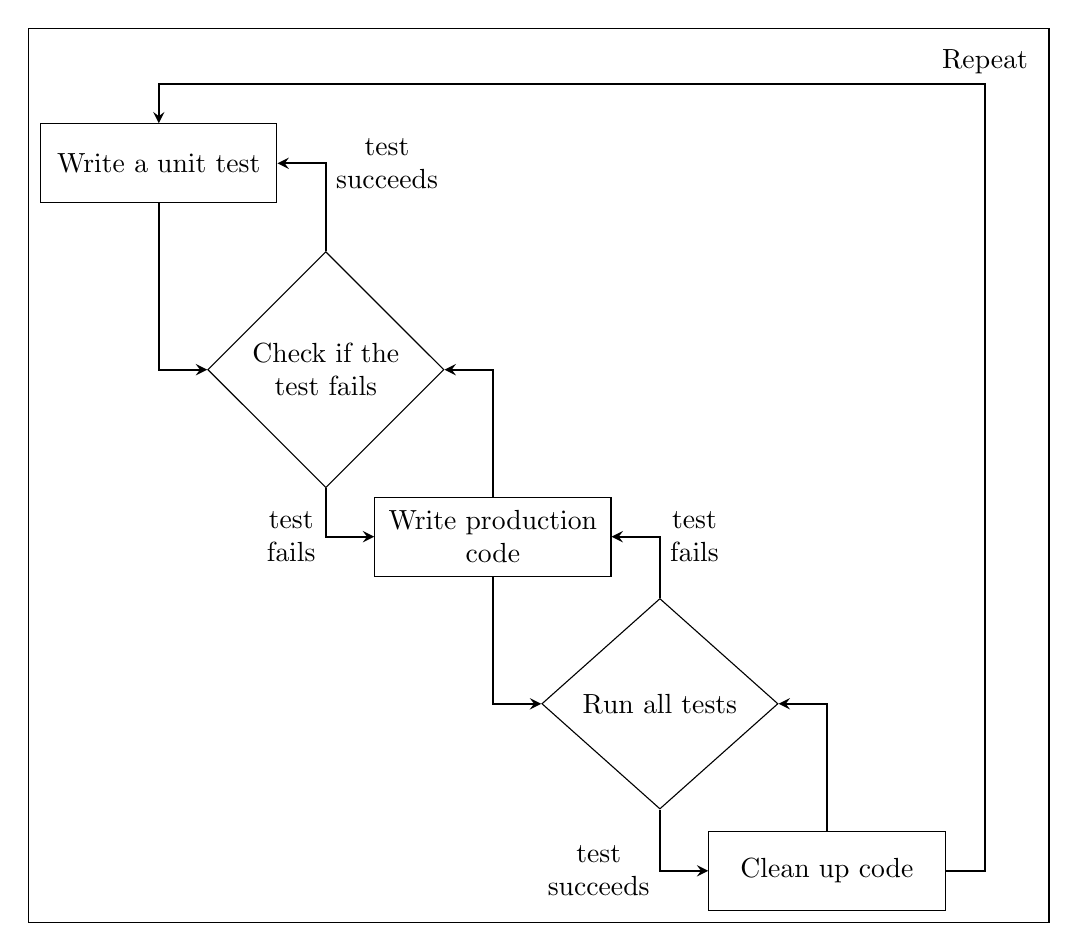
\begin{tikzpicture}[node distance=3cm, framed]
\node (start) [process] {Write a unit test};
\node (in1)[align=center] [decision, below right of=start, yshift=-0.5cm] {Check if the \\test fails};
\node (in2)[align=center] [process, below right of = in1] {Write production \\ code};
\node (in3)[align=center] [decision, below right of = in2] {Run all tests};
\node (in4)[align=center] [process, below right of = in3] {Clean up code};

\draw [arrow] (start) |- (in1);
\draw [arrow] (in1) |- node[anchor=west, align=center] {test \\succeeds} (start);
\draw [arrow] (in1) |- node[anchor=east, align=center] {test \\fails} (in2);
\draw [arrow] (in2) |- (in1);
\draw [arrow] (in2) |- (in3);
\draw [arrow] (in3) |- node[anchor=west, align=center] {test \\fails} (in2);
\draw [arrow] (in3) |- node[anchor=east, align=center] {test \\succeeds}(in4);
\draw [arrow] (in4) |- (in3);
\draw [arrow] (in4.east) -- ++(0.5,0) node(lowerright){}  |- node[anchor=south] {Repeat} ($(start.north)+(0,0.5)$) -- (start.north);
\end{tikzpicture}
\caption{The Test-Driven Development cycle}
\end{figure}


Unit Testing is generally synonymous with Test-Driven Development (TDD), where all tests are written before the api implementation begins. The tests are written based upon the api specification, thereby allowing any gaps in the specification to be discovered and filled in early. It also leads to less buggy software if done properly, as every module is sure to be unit tested. There are many tools to aid in trying to automate part of this process, some of which are discussed below.

\subsection{FitNesse}

FitNesse\footnote{\url{http://www.fitnesse.org}} is an acceptance testing framework\footnote{Unit tests written for the specific purpose of ensuring that the specification is fully implemented.}. It allows users to input formatted test cases, which it uses to automatically generates tests and execute them against the web api. While it generally works well when setup, it requires the creation of fixtures\footnote{Support classes with the api framework to allow the tests to run} which may be difficult depending on how the api is implemented. The test cases are created in a wiki using a natural language markup, which allows non-technical members of the team to also contribute to it.

FitNesse acts like a black-box test engine: the tester writing FitNesse inputs should not be aware how the specification is implemented. While a good idea in theory, there are usually bugs introduced due to the fixtures which can cause the acceptance tests to fail.  Furthermore, FitNesse is a completely self contained platform: it does not integrate with any other service, limiting furthermore automation.

\subsection{RSpec}

RSpec\footnote{\url{http://rspec.info}} is an acceptance testing framework for Ruby. It allows 'behaviours' to be defined which emulate a human using the api, and then automatically run against the code-base. It is by far the most commonly used testing framework for ruby apis, however it has seen limited use in other languages. Tests are written in a DSL based upon ruby which mimics natural language, making it easy to quickly add new tests as the need arises. Like FitNesse, RSpec is completely self contained and can not integrate with other services: the specification must be manually converted into behaviors.

\subsection{xUnit}

xUnit is a family of unit testing frameworks for object-oriented languages. They consist of seven major components:

\begin{tabular}{c  p{10cm}}
\textbf{Test runner} & Runs tests implemented using xUnit \\
\textbf{Test case} & Base class tests inherit from \\
\textbf{Test fixture} & Sets up the environment for a test. \\
\textbf{Test suite} & A set of tests that depend on the same fixture. \\
\textbf{Test execution} & Tests run an initializer, then the body of the test, and finish by cleaning up any changes they made. \\
\textbf{Test result formatter} & Interprets the results from the runner in a human readable format. \\
\textbf{Assertions} & A logical condition used to evaluate whether a test passed or failed. \\
\end{tabular}

xUnit frameworks are generally open source. This has allowed an ecosystem of services to develop around them, leading to easy integration of third party services. It is in active use by a wide variety of organizations, such as Microsoft\footnote{\url{http://www.nunit.org}} and Oracle\footnote{\url{http://junit.org}}. It is considered the industry standard in most enterprise application.

While powerful, xUnit frameworks again require the specification to be transformed into a propriety format. It can be very involved to setup, as fixtures need to be created for every test suite.


\subsection{Summary}

While there are a wast array of automatic testing tools, all of them require a large amount of manual intervention. Namely, all the tools discussed above require the original specification to be transformed into propriety formats. While this would not be an issue if this were to happen one, api specifications are continuously updated and so require an inordinate effort by the software engineer to keep the two models in sync. Furthermore, this is a likelihood of introducing errors when converting the specification to test cases.

An ideal solution would be able to parse a standardized specification and automatically generate all the relevant test cases, then execute the test cases against the code base. It would then be able to output which test cases failed in a human readable format.


\section{Livedrive}

Due to large possible scope of this project due to the myriad apis in production, I will limit the scope to an api provided by the organization Livedrive. Livedrive plan on using the completed project in production. They have begun created a new web api, code named 'Onyx', which can act as a good case study on how well the project will work in real world use cases.

Livedrive is a cloud backup company. They provide consumer facing clients which can be used to manage files. These files are then sent to an off-site server for storage, thereby allowing access from other clients and protecting them from machine failure. Onyx will be used to communicate between the clients and backend servers, allowing actions such as 'rename' and 'delete'. Onyx' is written in C\#, and is currently tested using FitNesse. Due to the quickly evolving nature of the api, FitNesse has proved too slow to be scalabe in the long term.

As Onyx is a trade secret, no code directly from the project will appear in the report. Instead, I will construct a mock api replicating the features of Onyx necessary to implement this project, as needed. This mock will aim to provide the same responses as Onyx, but will be merely imitating the responses.
% \chapter{Report Body}
The central part of the report usually consists of three or four chapters detailing the technical work undertaken during the project. {\bf{\textcolor{red}{The structure of these chapters is highly project dependent}}}. They can reflect the chronological development of the project, e.g. design, implementation, experimentation, optimisation, evaluation, etc (although this is not always the best approach). However you choose to structure this part of the report, you should make it clear how you arrived at your chosen approach in preference to other alternatives. In terms of the software that you produce, you should describe and justify the design of your programs at some high level, e.g. using OMT, Z, VDL, etc., and you should document any interesting problems with, or features of, your implementation. Integration and testing are also important to discuss in some cases. You may include fragments of your source code in the main body of the report to illustrate points; the full source code is included in an appendix to your written report.

\section{Section Heading}

\subsection{Subsection Heading}
\chapter{Requirements}

Below are a set of functional and non-functional requirements based upon which the system should be developed. Successful completion of this project should lead to a well defined way of specifing restful web apis, and using this specifcation to automatically test the implementation for bugs.

\section{User Requirements}

This section defines all the actions a user must be able to perform:

\begin{itemize}
\item Fully specify a restful web api, so that it can be clearly understood by developers and software architects.
\item Be able to define what 'correct' operation of the api results in.
\item Automatically run tests against an implementation of the web api based upon the specification.
\item Be able to define sample inputs for the restul web api.
\item Be able to define sample outputs for a given input.
\item Be able to check in the api returns the correct output for any given input.
\end{itemize}

\section{Functional Requirements}

This section defines the functionality the system must be able to accomplish.

\begin{itemize}
\item Parse the specification into a machine readable format.
\item Provide the user with a method to execute tests against a web api.
\item Report to the user how many tests failed.
\item Be able to send sample inputs to the restful api and ensure they are valid.
\item Be able to detect if an api implementation does not follow the specification.
\end{itemize}

\section{Non-Functional Requirements}

This section defines more subjective requirements which will help provide a high quality project. It is split into two parts: Specification and Automated testing.

\subsection{Specification}
\begin{itemize}
\item The specification language must be easily human readable.
\item The language must be able to suiccintly and unambiuously define a restful web api.
\item The language must be easily convertable to a format machines can process.
\item The language most be agnostic to any implementation details. It should not matter how the api is going to work, or which programming language it will be written in.
\end{itemize}

\subsection{Automated testing}
\begin{itemize}
\item The system should be reliable: it should return the same result if run with the same specification on the same implementatiom.
\item The system should be implementation agnostic: It should be able to run the tests no matter what language the api is written in.
\item The system should be able to run on as many common operating systems as feasibly possible.
\item The system should be performant, scaling linearly with the number of tests being run.
\item The system shpuld be easy to maintain, following development best practices and making good use of architecturel design patterns.
\item The system should be fully unit tested to provide assurences that the code is as correct as possible.
\end{itemize}
% \chapter{Design Considerations}

This chapter discusses the overall system design of the project, and details what each module of the system will accomplish. The chapter will give a high level overview, with more in depth implementation details further on. Each choice is based upon achieving one of the requirement of the project

\section{Requirements}

Below are a set of functional and non-functional requirements based upon which the system should be developed. Successful completion of this project should lead to a well defined way of specifying restful web APIs, and using this specification to automatically test the implementation for bugs.

\subsection{User Requirements}

This section defines all the actions a user must be able to perform:

\begin{itemize}
\item Fully specify a restful web API, so that it can be clearly understood by developers and software architects.
\item Be able to define what 'correct' operation of the API results in.
\item Automatically run tests against an implementation of the web API based upon the specification.
\item Be able to define sample inputs for the restful web API.
\item Be able to define sample outputs for a given input.
\item Be able to check in the API returns the correct output for any given input.
\end{itemize}

\subsection{Functional Requirements}

This section defines the functionality the system must be able to accomplish.

\begin{itemize}
\item Parse the specification into a machine readable format.
\item Provide the user with a method to execute tests against a web API.
\item Report to the user how many tests failed.
\item Be able to send sample inputs to the restful API and ensure they are valid.
\item Be able to detect if an API implementation does not follow the specification.
\end{itemize}

\subsection{Non-Functional Requirements}

This section defines more subjective requirements which will help provide a high quality project. It is split into two parts: Specification and Automated testing.

\subsubsection{Specification}
\begin{itemize}
\item The specification language must be easily human readable.
\item The language must be able to succinctly and unambiguously define a restful web API.
\item The language must be easily convertible to a format machines can process.
\item The language most be agnostic to any implementation details. It should not matter how the API is going to work, or which programming language it will be written in.
\end{itemize}

\subsubsection{Automated testing}
\begin{itemize}
\item The system should be reliable: it should return the same result if run with the same specification on the same implementation.
\item The system should be implementation agnostic: It should be able to run the tests no matter what language the API is written in.
\item The system should be able to run on as many common operating systems as feasibly possible.
\item The system should be performant, scaling linearly with the number of tests being run.
\item The system should be easy to maintain, following development best practices and making good use of architectural design patterns.
\item The system should be fully unit tested to provide assurances that the code is as correct as possible.
\end{itemize}

\section{System Components}

The project consists of three overall systems, which can be broken down into smaller modules.

\textbf{The RATML specification:} A high level specification language based upon RAML, allowing restful web APIs to be fully specified. The language can be split into two parts:
\begin{itemize}
\item A language to define the endpoints of the API, along with all of its collections and resources. An API should be able to be implemented using just this as an reference.
\item A language to define test input and output data.
\end{itemize}

\textbf{RATML parser:} As RATML is a new specification language, a custom parser will need to be built.
\begin{itemize}
\item A YAML parser will be used to convert the text based specification file into a human processable format.
\item A RATML parser will then take as input the objects from the YAML parser, and convert them into a data structure that can be used by the rest of the system.
\item A facade will allow the system to quickly query and manipulate the aforementioned data structure.
\end{itemize}

\textbf{RATML Framework}: The framework will use the parsed data to create and execute tests.
\begin{itemize}
\item A system to iterate through the endpoints and generate the best possible test for it.
\item A system to use the sample input data to interpolate more possible values for the endpoint, and use it to send test requests.
\item A system to report the discovered results in a human readable manner.
\end{itemize}

The big advantage of this approach is the separation of concerns: each of the three components is loosely linked and therefore can be worked on and tested in isolation.

\begin{figure}[ht]
\begin{tikzpicture}[node distance=3.5cm, framed]
\node (spec) [process] {Specification};
\node (API) [process, below left of=spec] {Web API};
\node (parser) [process, below right of = spec] {Parser};
\node (test) [process, below right of = API] {Test Framework};

\node (ratml) [process, right of = parser, xshift = 0.5cm] {RATML Parser};
\node (yaml) [process, above of = ratml, yshift = -1.75cm] {YAML Parser};
\node (facade) [process, below of = ratml, yshift = 1.75cm] {Facade};
\node (model) [process, right of = ratml] {Model};
\node [draw=black, fit= (ratml) (yaml) (facade) (model), dashed] {};

\node (exec) [process, below of = test, yshift = 1.25cm] {Execute Tests};
\node (gen) [process, left of = exec] {Generate Tests};
\node (dis) [process, right of = exec] {Report Results};
\node [draw=black, fit= (gen) (exec) (dis), dashed] {};

\draw [arrow] (spec) -- node[anchor=west, align=center] {Definition} (parser);
\draw [arrow] (parser) -- (test);
\draw [arrow] (test) -- (API);
\draw [arrow] (spec) -- node[anchor=east] {Implementation}(API);

\draw [arrow] (parser) -- (yaml);
\draw [arrow] (yaml) -- (ratml);
\draw [arrow] (ratml) -- (model);
\draw [arrow] (model) -- (facade);
\draw [arrow] (facade) -- (parser);

\draw [arrow] (test) -- (gen);
\draw [arrow] (gen) -- (exec);
\draw [arrow] (exec) -- (dis);
\draw [arrow] (dis) -- (test);
\end{tikzpicture}
\caption{System Architecture Diagram}
\end{figure}

\section{Software Packages}

The system will mainly be written in Ruby\footnote{\url{https://www.ruby-lang.org}}. This is due to the language's prominence in the Test Driven Development committee, along with being multi-platform. The language comes pre-installed on OS X and most distributions of Linux, as well as being easily installable on Windows, thereby covering the three biggest browsers. Furthermore, the language is completely portable, and the same code base works on any supported platform. Of particular note are the languages meta-programming capabilities, which allow parsers to be written very efficiently.

In particular, Ruby's Blocks are an implementation of higher level functions which allow arbitrary code to be stored as variables and passed around the system. This allows for code to be very highly encapsulated,  such as letting the test framework generate and execute tests on the fly. I will use the Sublime Text editor to write the code, which is freely available\footnote{\url{https://www.sublimetext.com}}.

\section{Testing}

As the main code-base will be written in Ruby, the Onyx imitation will also be written in the same language for consistency. Therefore, I will use the Ruby on Rails\footnote{\url{http://rubyonrails.org}} library. This library is specifically designed for creating web services, and provides many features to aid in this. Some of these includes a routing table to direct API requests and tight integration with a SQL database to store collections, along with support for all HTTP Verbs/

Rails applications come bundled with a server to quickly set up and host the web service, thereby allowing very fast iterations on the API implementation.
% \chapter{Implementation}

\section{Section Heading}

% \chapter{Professional and Ethical Issues}
Either in a seperate section or throughout the report demonstrate that you are aware of the \textbf{Code of Conduct \& Code of Good Practice} issued by the British Computer Society and have applied their principles, where appropriate, as you carried out your project.

\section{Section Heading}

% \chapter{Evaluation}

This section will analyze the completed system based upon the previously stated functional and non-functional requirements, as well as competing solutions on the market.

\section{Requirements}

To ensure that the system has been developed according to the problem laid out at the start of this thesis, it will be evaluated against the requirements outlined earlier.

\subsection{User Requirements}

\begin{itemize}
\item \emph{Fully specify a restful web API, so that it can be clearly understood by developers and software architects.} Restful APIs can be fully specified using RATML. Whether it can be clearly understood by developers is subjective, however it is based upon RAML which is widely used, and so it is safe to assume that the language is clear. Livedrive have begun using RATML, further pointing towards the language being useful.
\item \emph{Be able to define what 'correct' operation of the API results in.} This was accomplished using schema definition for responses, which can be evaluated against the API implementation. While not perfect - it is possible to create a response which matches the schema but is not valid - it has a ~98\% rate when the heuristic is fed some seed data. This is an area which could use improvement in the future, but suffices for current use.
\item \emph{Automatically run tests against an implementation of the web API based upon the specification.} This was accomplished using the Test Generation and Execution modules: Test cases are created from a RATML specification. They are sent as requests to the API implementation, and the responses evaluated for correctness. Results can then be reported to the user if a human-readable format.
\item \emph{Be able to define sample inputs for the restful web API. / Be able to define sample outputs for a given input.} The RATML extensions to add Test Cases allow multiple inputs and outputs to be defined for each method in a restful API.
\item \emph{Be able to check in the API returns the correct output for any given input.} The RATML parser was extended to be able to process Test Cases and transform them into the same format already being used by the Test Execution module.
\end{itemize}

\subsection{Functional Requirements}

\begin{itemize}
\item \emph{Parse the specification into a machine readable format.} A YAML parser was modified to act as a RATML parser, thereby fulfilling this requirement. The parser outputs ruby Objects which can be easily processed by a computer, as well as providing a Facade for easy manipulation by other modules.
\item \emph{Provide the user with a method to execute tests against a web API.} The command-line interface allows the user to select a RATML file and begin test execution against its implementation.
\item \emph{Report to the user how many tests failed.} The pretty printer can process the test result objects and output how many tests failed, along with many other useful information for the user.
\item \emph{Be able to send sample inputs to the restful API and ensure they are valid.} Test Cases can be sent to the API implementation using the Typhoeus library, and the completion handler closures evaluate if the response is valid.
\item \emph{Be able to detect if an API implementation does not follow the specification.} The existence and schema checks carried out by the Test Execution module ensure that endpoints are implemented, while the input/output tests can be used for more nuanced probing.
\end{itemize}

\subsection{Non-Functional Requirements}

\subsubsection{Specification}
\begin{itemize}
\item \emph{The specification language must be easily human readable. / The language must be able to succinctly and unambiguously define a restful web API.} As discussed above, these are subjective requirements. RATML is now being used at Livedrive by several engineers and has yet to receive any complaints about it's design, so this requirement can be considered to be met.
\item \emph{The language must be easily convertible to a format machines can process.} RATML is based upon YAML, which is a very mature markup language with many parsers available.  While RATML specific parser will have to be written, such as the ruby based one created for this thesis, the process can be drastically simplifies by using an existing YAML parser as the code base.
\item \emph{The language most be agnostic to any implementation details. It should not matter how the API is going to work, or which programming language it will be written in.} RATML can specify APIs which are then implemented in any language: there are no language specific features within it.
\end{itemize}

\subsubsection{Automated testing}
\begin{itemize}
\item \emph{The system should be reliable: it should return the same result if run with the same specification on the same implementation.} Due to the added dependency features, tests are run in a non-destructive order allowing the system to be reliable.
\item \emph{The system should be implementation agnostic: It should be able to run the tests no matter what language the API is written in.} Test cases are executed as network requests, and therefore do not need to know any implementation details of the API.
\item \emph{The system should be able to run on as many common operating systems as feasibly possible.} The system is written in ruby, allowing the same code base to be run on OS X, Windows, most Linux distributions and many other platforms\footnote{\url{https://bugs.ruby-lang.org/projects/ruby-trunk/wiki/20SupportedPlatforms}}.
\item \emph{The system should be performant, scaling linearly with the number of tests being run.} Thanks to the parallelized design, the system is highly performant, regularly scaling faster than linearly depending on the number of cpu cores available. 
\item \emph{The system should be easy to maintain, following development best practices and making good use of architectural design patterns.} The system is highly modular. There are two major components: the parser and the test framework, both of which are further split into components. There is ample documentation throughout, and the Model-View Controller design pattern is followed. Individual components can be modified or replaced without breaking the overall system.
\item \emph{The system should be fully unit tested to provide assurances that the code is as correct as possible.} Every module has unit tests, all of which pass. A sample 'Onyx' API was implemented to model real world usage, and the test framework behaves as expected when executed against it.
\end{itemize}

\subsection{Conclusion}

While there are a few small areas where improvement is possible, the system generally meets all the requirements laid out at the start. Of particular note is the fact that defining a 'correct' API proved difficult: it is a concept easily understood by humans but can not be simply specified in a machine-computable format. Nevertheless, the input-output test cases can help cover this deficiency and the 98\% success rate isn't unusable.

\section{Current Solutions}

As covered in the Background, there are existing products also aiming at automating testing. This section compares the effectiveness of existing solutions to RATML and the Test Framework developed here.

\subsection{RAML}

While RATML is heavily based upon RAML, they are not the same. Both languages are built on top of YAML, thereby allowing them to be easily parsed. RATML has been simplified, allowing specialized parsers to be easier to write, as shown by the fully working RATML parser which I managed to implement, in contrast to the abandoned Ruby RAML parser. On the other hand, RAML possesses many abstraction techniques such as traits that allow more concise specifications to be written, whereas RATML requires everything to be explicitly laid out. While this gives RAML a higher difficulty curve to learn, it allows specifications to be much more easily followed by humans. RATML allows the definitions of input/output test cases. RAML partially supports this in the form of examples, however the RATML implementation is far more robust, allowing automatic test generation from the Test Case definitions.

As RAML and RATML target different use cases, one can not be said to definitely be better than the other. One major advantage that RAML possesses is the already existing third-party resources and industry backing. Convincing the market to learn a new specification language and rewrite the many existing tools is a difficult task, especially as RAML has a large corporation backing it. However, as shown by the lack of automatic test tooling, RAML \emph{is} limited when it comes to test generation, and this is the use case where RATML clearly wins out.

\subsection{FitNesse}

FitNesse is the test suite most similar to this project. It consists of a wiki-type file used to specify inputs and outputs. The wiki file is then used to generate test cases, and ran against the api implementation. Like RAML, FitNesse has the advantage of existing tooling and industry support. FitNesse and the Test Framework both allow tests to be specified in a human readable manner, then parsed and run by the computer. FitNesse requires prior setup by a software engineer, while the Test Framework can be executed directly: it only needs a RATML file as input. Furthermore, the Test Framework can do presence and schema checks which FitNesse can not - it requires an exact output for any input.

This project's major advantage over FitNesse is ease of use. The specification can be automatically converted into test cases, input does not need to be specified in a special file. Furthermore, FitNesse requires the creation of Mocks and Fixtures to operate properly. The entire api code base must be modified to be compatible with FitNesse while the Test Framework can work 'out of the box.' On the other hand, once Mocks and Fixtures are created, FitNesse allows for a far wider variety of test cases to be written. The Test Framework requires the API implementation to be set up with a test database, while FitNesse can automatically populate with API with mock data. The Test Framework tests the implementation as a whole, while FitNesse can target individual modules.

All in all, the Test Framework provides simple, fully automated test cases. FitNesse can provide more control, at the cost of required manually integration. Both systems can be used as required by a project.

\section{Livedrive and Onyx}

The imitation Onyx API was run against the Test Framework. The results were encouraging: all the tests passed, showing that RATML \emph{can} be used to fully specify an API, and create automatic tests for it. 

I also ported the entire Onyx specification definition to RATML, and ran it against the Test Framework. The complete specification has 403 endpoints and just under 5000 test cases. Of these, close to 4000 can be processed by the test Framework. Issues were caused by cases related to authorization and authentication, which were omitted from the imitation API due to trade secrets. While the Test Framework can handle most authorization techniques, it can not handle OAUTH\cite{rfc6749} due to the multiple redirects involved.

\begin{tabular}{c | c | c}
& \textbf{Imitation} & \textbf{Onyx} \\ \hline
\textbf{Endpoints} & 10 & 403 \\ \hline
\textbf{Input/Output Cases} & 40 & 4989 \\
\textbf{Successful Tests} & 40 & 3890 \\ \hline
\textbf{Schema Tests} & 21 & 10211 \\
\textbf{Successful Schema Tests} & 20 & 10007 \\ \hline 
\textbf{Time to run Tests} & 31ms & 5131ms \\
\end{tabular}

Discussing the Test Framework with Livedrive engineers, the general consensus is that the system is best in class for it's use case, and RATML is a very nice language to write specifications in. However, it is not fully featured enough to be a complete replacement, and thus will be used alongside FitNesse for the time being. The Test Framework is open source, and I will continue working on it as an employee of Livedrive when this thesis is finished. Livedrive is already starting to implement it as part of their test process, showing that the project meets a need in the industry.
% \chapter{Conclusion and Future Work}

There are a myriad ways of testing an application, and automating all of them is difficult, arguably impossible. This thesis set out to tackle a subset of the tests currently manually conducted in software engineering companies, and I believe it has satisfactorily met this challenge. RATML provides an unambiguous, human and machine readable format for defining restful web APIs, while the Test Framework can transform the specification into a suite of varied tests. The tests can be executed against an implementation of the API, and the results reported to the user. By using popular, open source projects like YAML and ruby as a basis, the project has a good chance of catching on in the industry, and has already been adopted by Livedrive. 

The project is obviously not a complete system. Tests are limited to three major categories: Presence, schema and input/output. There are far more possible such as integration, component and functional. Furthermore, scheme test do not yet have a 100\% reliability rate, though I do not believe there are any other systems on the market which even attempt schema tests.

RATML and the Test Framework are centred around restful web APIs. While the Test Framework is generic enough that it could conceivably function with other restful services, RATML certainly can not and would need major expansion. These limitations mean that the project is currently only a viable solution for Livedrive and similar companies: it can not be used for other types of applications.

While the requirements for this thesis have been met, I will continue work on the Test Framework. Future extensions include adding support for Mocks and Fixtures. The Framework is currently limited to testing the API implementation as a whole, which is not always beneficial. A heuristic to determine components from the specification and target tests accordingly could help the Test Framework replace FitNesse.

RATML can also be improved. RAML contains constructs to define security mechanisms, and abstraction layers to allow the specification to be split over several files. These can be ported to RATML and implemented in the parser, allowing greater interoperability between RATNL and RAML.

Thanks to it's parallelized design, the application is highly scalable. While it is fast enough for it's current uses, there are several ways to gain more performance from it. The parser can be written in a lower-level, compiled language to speed up RATML parsing. While ruby has proven fast enough so far thanks to manipulating the YAML syntax tree directly, it has been at the cost of increasing memory usage. Writing the entire parser in C++ or Rust could help with this if it ever becomes a bottleneck.

The biggest roadblock for RATML and the Test Framework is adoption. Test suites do not live in isolation, and must consist of an ecosystem to be truly useful. Therefore, the entire project will be open sourced to encourage the community to contribute and improve it. However, it is competing with the already ingrained RAML and FitNesse. The Test Framework meets a specific niche, and that may help it be used alongside other products while the ecosystem builds.

%%%%%%%%%%%%%%%%%%%%%%%%%%%%%%%%%
% References
%%%%%%%%%%%%%%%%%%%%%%%%%%%%%%%%%
\bibliographystyle{plain}
\bibliography{references}
\addcontentsline{toc}{section}{Bibliography}

%%%%%%%%%%%%%%%%%%%%%%%%%%%%%%%%%
% Appendices
%%%%%%%%%%%%%%%%%%%%%%%%%%%%%%%%%
\appendix
\include{Appendices/appendix}
\chapter{User Guide}
\section{Instructions}
You must provide an adequate user guide for your software. The guide should provide easily understood instructions on how to use your software. A particularly useful approach is to treat the user guide as a walk-through of a typical session, or set of sessions, which collectively display all of the features of your package. Technical details of how the package works are rarely required. Keep the guide concise and simple. The extensive use of diagrams, illustrating the package in action, can often be particularly helpful. The user guide is sometimes included as a chapter in the main body of the report, but is often better included in an appendix to the main report.

\chapter{Source Code}
\section{Instructions}
Complete source code listings must be submitted as an appendix to the report. The project source codes are usually spread out over several files/units. You should try to help the reader to navigate through your source code by providing a ``table of contents'' (titles of these files/units and one line descriptions). The first page of the program listings folder must contain the following statement certifying the work as your own: ``I verify that I am the sole author of the programs contained in this folder, except where explicitly stated to the contrary''. Your (typed) signature and the date should follow this statement.

All work on programs must stop once the code is submitted. You are required to keep safely several copies of this version of the program - one copy must be kept on the departmental disk space - and you must use one of these copies in the project examination. Your examiners may ask to see the last-modified dates of your program files, and may ask you to demonstrate that the program files you use in the project examination are identical to the program files you had stored on the departmental disk space before you submitted the project. Any attempt to demonstrate code that is not included in your submitted source listings is an attempt to cheat; any such attempt will be reported to the KCL Misconduct Committee.

\textbf{You may find it easier to firstly generate a PDF of your source code using a text editor and then merge it to the end of your report. There are many free tools available that allow you to merge PDF files.}


\end{document}
